\documentclass{scrartcl}

\usepackage{Packages_Makros}

\MyTitle{Portfolio}
\MySubtitle{Die Energiewirtschaft}
\MyAuthor{Felix Hehemann}
\MyEmail{felix.hehemann@fh-muenster.de}
\MyMatrNo{1250378}
\MyDepartment{Energie Gebäude Umwelt}
\MyFirstExaminer{Prof. Dr. Peter Vennemann}

\begin{document}

\myMakeTitlepage

\section{Energienutzung in der Zivilisationsgeschichte}
    \begin{figure}[H]
    \centering
    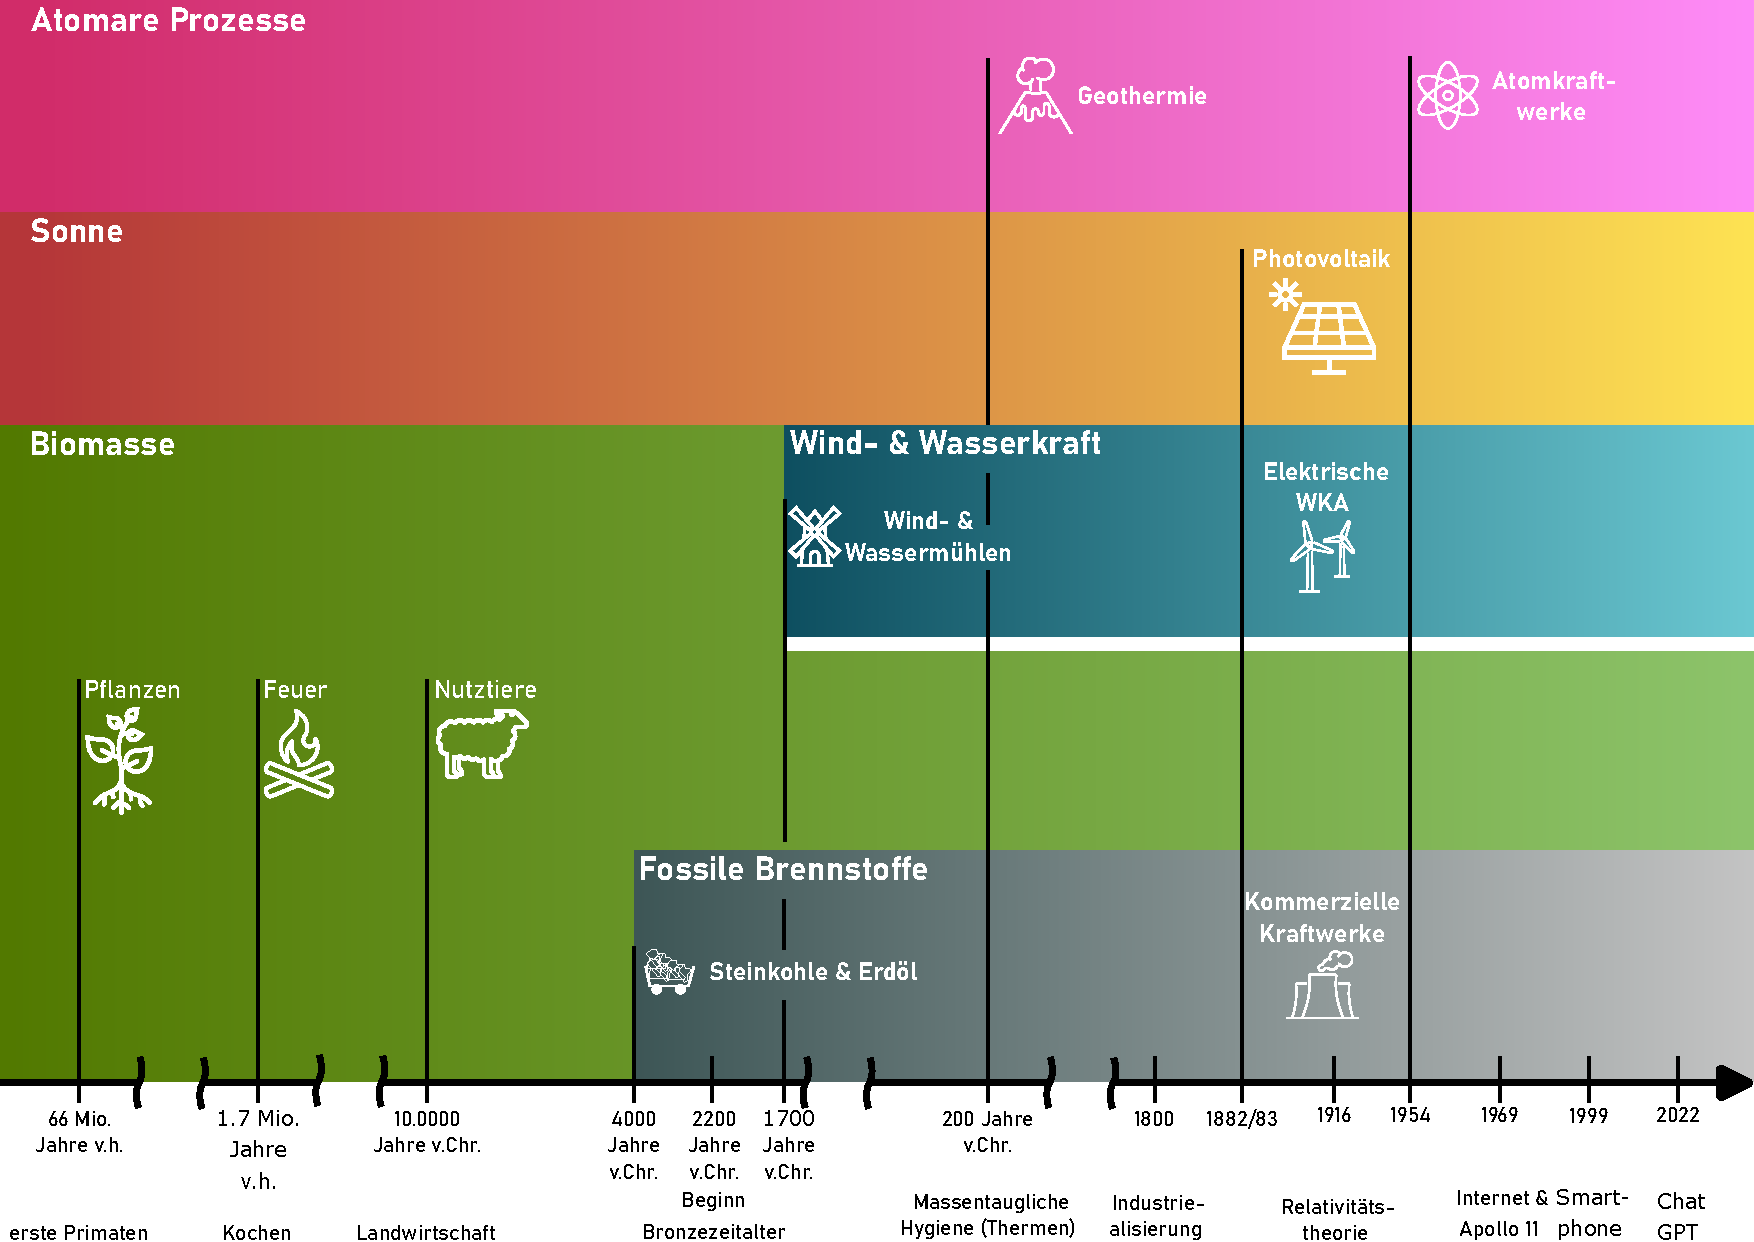
\includegraphics[width=1\linewidth]{Abbildungen/Zivilisation_Energie.pdf}
    \caption[Genutzte Energiequellen in der Zivilisationsgeschichte]{Die Abbildung 
    zeigt unterschiedliche genutzte Energiequellen in der Zivilisationsgeschichte 
    der Menschheit sowie Zusammenhänge mit technischem und gesellschaftlichem Fortschritt. 
    Aus dem hierarchischen Aufbau wird deutlich, dass mit wachsendem Fortschritt immer mehr 
    und höherwertige Quellen erschlossen wurden. Quellen(s. Tabelle \ref{tab:Energiegeschichte})}
    \label{fig:Energienutzung}
\end{figure}

\begin{table}[H]
    \centering
    \begin{tabular}{c|p{10 cm}}
         Ereignis &  Quelle  \\
         \hline
        erste Primaten & \url{ https://geoundnatur.de/Documents/geologische-zeitskala.pdf} \\
        \hline
        Pflanzen & \url{https://geoundnatur.de/Documents/geologische-zeitskala.pdf}  \\
        \hline
        Feuer & \url{https://doi.org/10.1086/203705}, \url{https://doi.org/10.1073/pnas.1117620109} \\
        \hline
        Kochen & \url{https://doi.org/10.1073/pnas.1107806108} \\
        \hline
        Nutztiere & \url{https://www.youtube.com/watch?v=xiYMWSA3s\_A} \\
        \hline
        Wind- \& Wassermühlen & Golding, E. W. (1976). The Generation of Electricity by the Wind, reprinted with additional material by E. \& FN Spon.; Quaschning, V. (2015). Regenerative Energiesysteme: Technologie-Berechnung-Simulation. Carl Hanser Verlag GmbH Co KG. \\
        \hline
        Steinkohle- \& Erdölnutzung & \url{https://10.1126/sciadv.adh0549} \\
        Bronzezeitalter -\& & \url{https://geoundnatur.de/Documents/geologische-zeitskala.pdf} \\ 
        Geothermie & Bundesverband Geothermie \\
        \hline
        Industrialisierung & \url{https://de.wikipedia.org/wiki/Industrialisierung}  \\ 
        \hline
        Kommerzielle Kraftwerke & Wolter, D., \& Reuter, E. (2005). Preis-und Handelskonzepte in der Stromwirtschaft: von den Anfängen der Elektrizitätswirtschaft zur Einrichtung einer Strombörse. Springer-Verlag. \\
        \hline
        Elektrische WKA & \url{https://www.e-rara.ch/zut/22499137 }\\
        \hline
        Photovoltaik & \url{https://doi.org/10.2475/ajs.s3-26.156.465} \\
        \hline
        Relativitätstheorie & \url{https://doi.org/10.1007/978-3-540-87777-6\_1}\\
        \hline
        Atomkraftwerke &  \url{https://www.iaea.org/newscenter/news/obninsk-beyond-nuclear-power-conference-looks-future}\\
        \hline
        Internet \& Apollo 11 & \url{https://www.nasa.gov/mission/apollo-11/}; \url{https://www.deutschlandfunk.de/erste-nachricht-im-arpanet-vor-50-jahren-als-der-100.html}\\
        \hline
        Chat GPT & \url{https://openai.com/de-DE/index/chatgpt/}
    \end{tabular}
    \caption{Quellen zu \ref{fig:Energienutzung}}
    \label{tab:Energiegeschichte}
\end{table}

\section{Kumulativer Energie Aufwand}
Die Berechnung des kumulativen Energie Aufwands wird dazu verwendet um
einen vergleichbaren Rahmen zu schaffen um Produkte hinsichtlich ihrer Energie-
und Ressourceneffizienz zu bewerten. Dabei werden energietechnische Daten in
einem einheitlichen Rahmen vergleichbar gemacht. (Quellen siehe \ref{tab:KEA})

\begin{figure}[h]
    \centering
    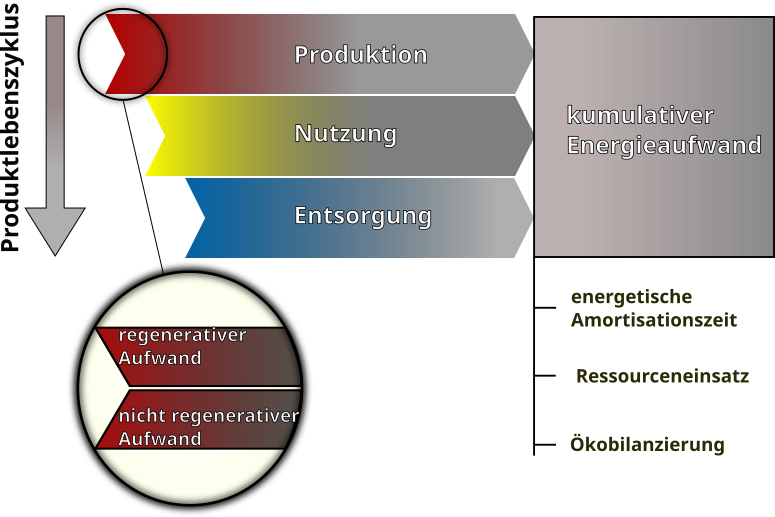
\includegraphics[width=0.8\textwidth]{Abbildungen/KEA.png}
    \caption{Zusammensetzung des Kumulativen Energiebedarfs nach VDI 4600:2012-01. 
    Anhand der einheitlichen Primärenergetischen Betrachtung lassen sich Produkte 
    hinsichtlich ökologischer und energetischer Sicht bewerten und vergleichen. 
    Der Bilanzraum liegt um den gesamten Produktlebenszyklus bzw. um die einzelnen
    Teilschritten Produktion, Nutzung, Entsorgung. Quellen(s. Tabelle \ref{tab:KEA})}
    \label{fig:KEA}
\end{figure}

\begin{table}[h]
    \centering
    \begin{tabular}{c|c}
        \textbf{Quelle} & textbf{Link} \\ \hline
        VDI 4600 & \url{www.dinmedia.de/de/technische-regel/vdi-4600/143521324}
    \end{tabular}
    \caption{Quellen zu \ref{fig:KEA}}
    \label{tab:KEA}
\end{table}

\section{Carnot Batterie}

In der Literatur werden Carnot-Batterien als eine Zukunftstechnologie der 
Energiespeicherung angepriesen, mit welcher es möglich sein soll Wirkungsgrade von über 
\SI{100}{\percent} erreichen. Abbildung \ref{fig:CarnotBatterie} zeigt einen Aufbau, mit dem eine 
Power to Power Effizienz von 1,06 erreicht werden soll. Wie ist das möglich, wenn 
doch nach dem zweiten Hauptsatz der Thermodynamik, der maximal arbeitsfähige Anteil 
thermischer Energie durch den Carnot Wirkungsgrad begrenzt ist? Wird hier die Thermodynamik 
ausgetrickst? Die Antwort ist, nein. Schaut man sich das System genauer an, sieht man, dass 
die Systemgrenze offen ist. Die Carnot Batterie aggiert mit Ihrer Umwelt und es wird neben Strom 
auch Abwärme in das System mit eingespeißt. Mit Hilfe einer Stromgetriebenen Wärmepumpe 
auf der einen Seite wird das Temperaturniveau der Abwärme effizient angehoben, dann in einem 
Wärmespeicher zwischengespeichert und bei Bedarf von einer Wärmekraftmaschine in 
Strom gewandelt. Alle Prozesse sind Verlustbehaftet. Durch das stetige hinzufügen von 
Abwärme werden diese Verluste jedoch scheinbar kompensiert. Schaut man sich dann 
nur die elektirschen Anteile des Systems an wirkt es so, als hätte das System eine 
positive Bilanz. Werden alle Energieanteile berücksichtigt muss man jedoch feststellen, 
dass das System zwar die Abwärme effizient nutzbar macht, aber weiterhin Verlusten 
nach dem Carnot Wirkungsgrad unterliegt. 

\begin{figure}[h]
    \centering
    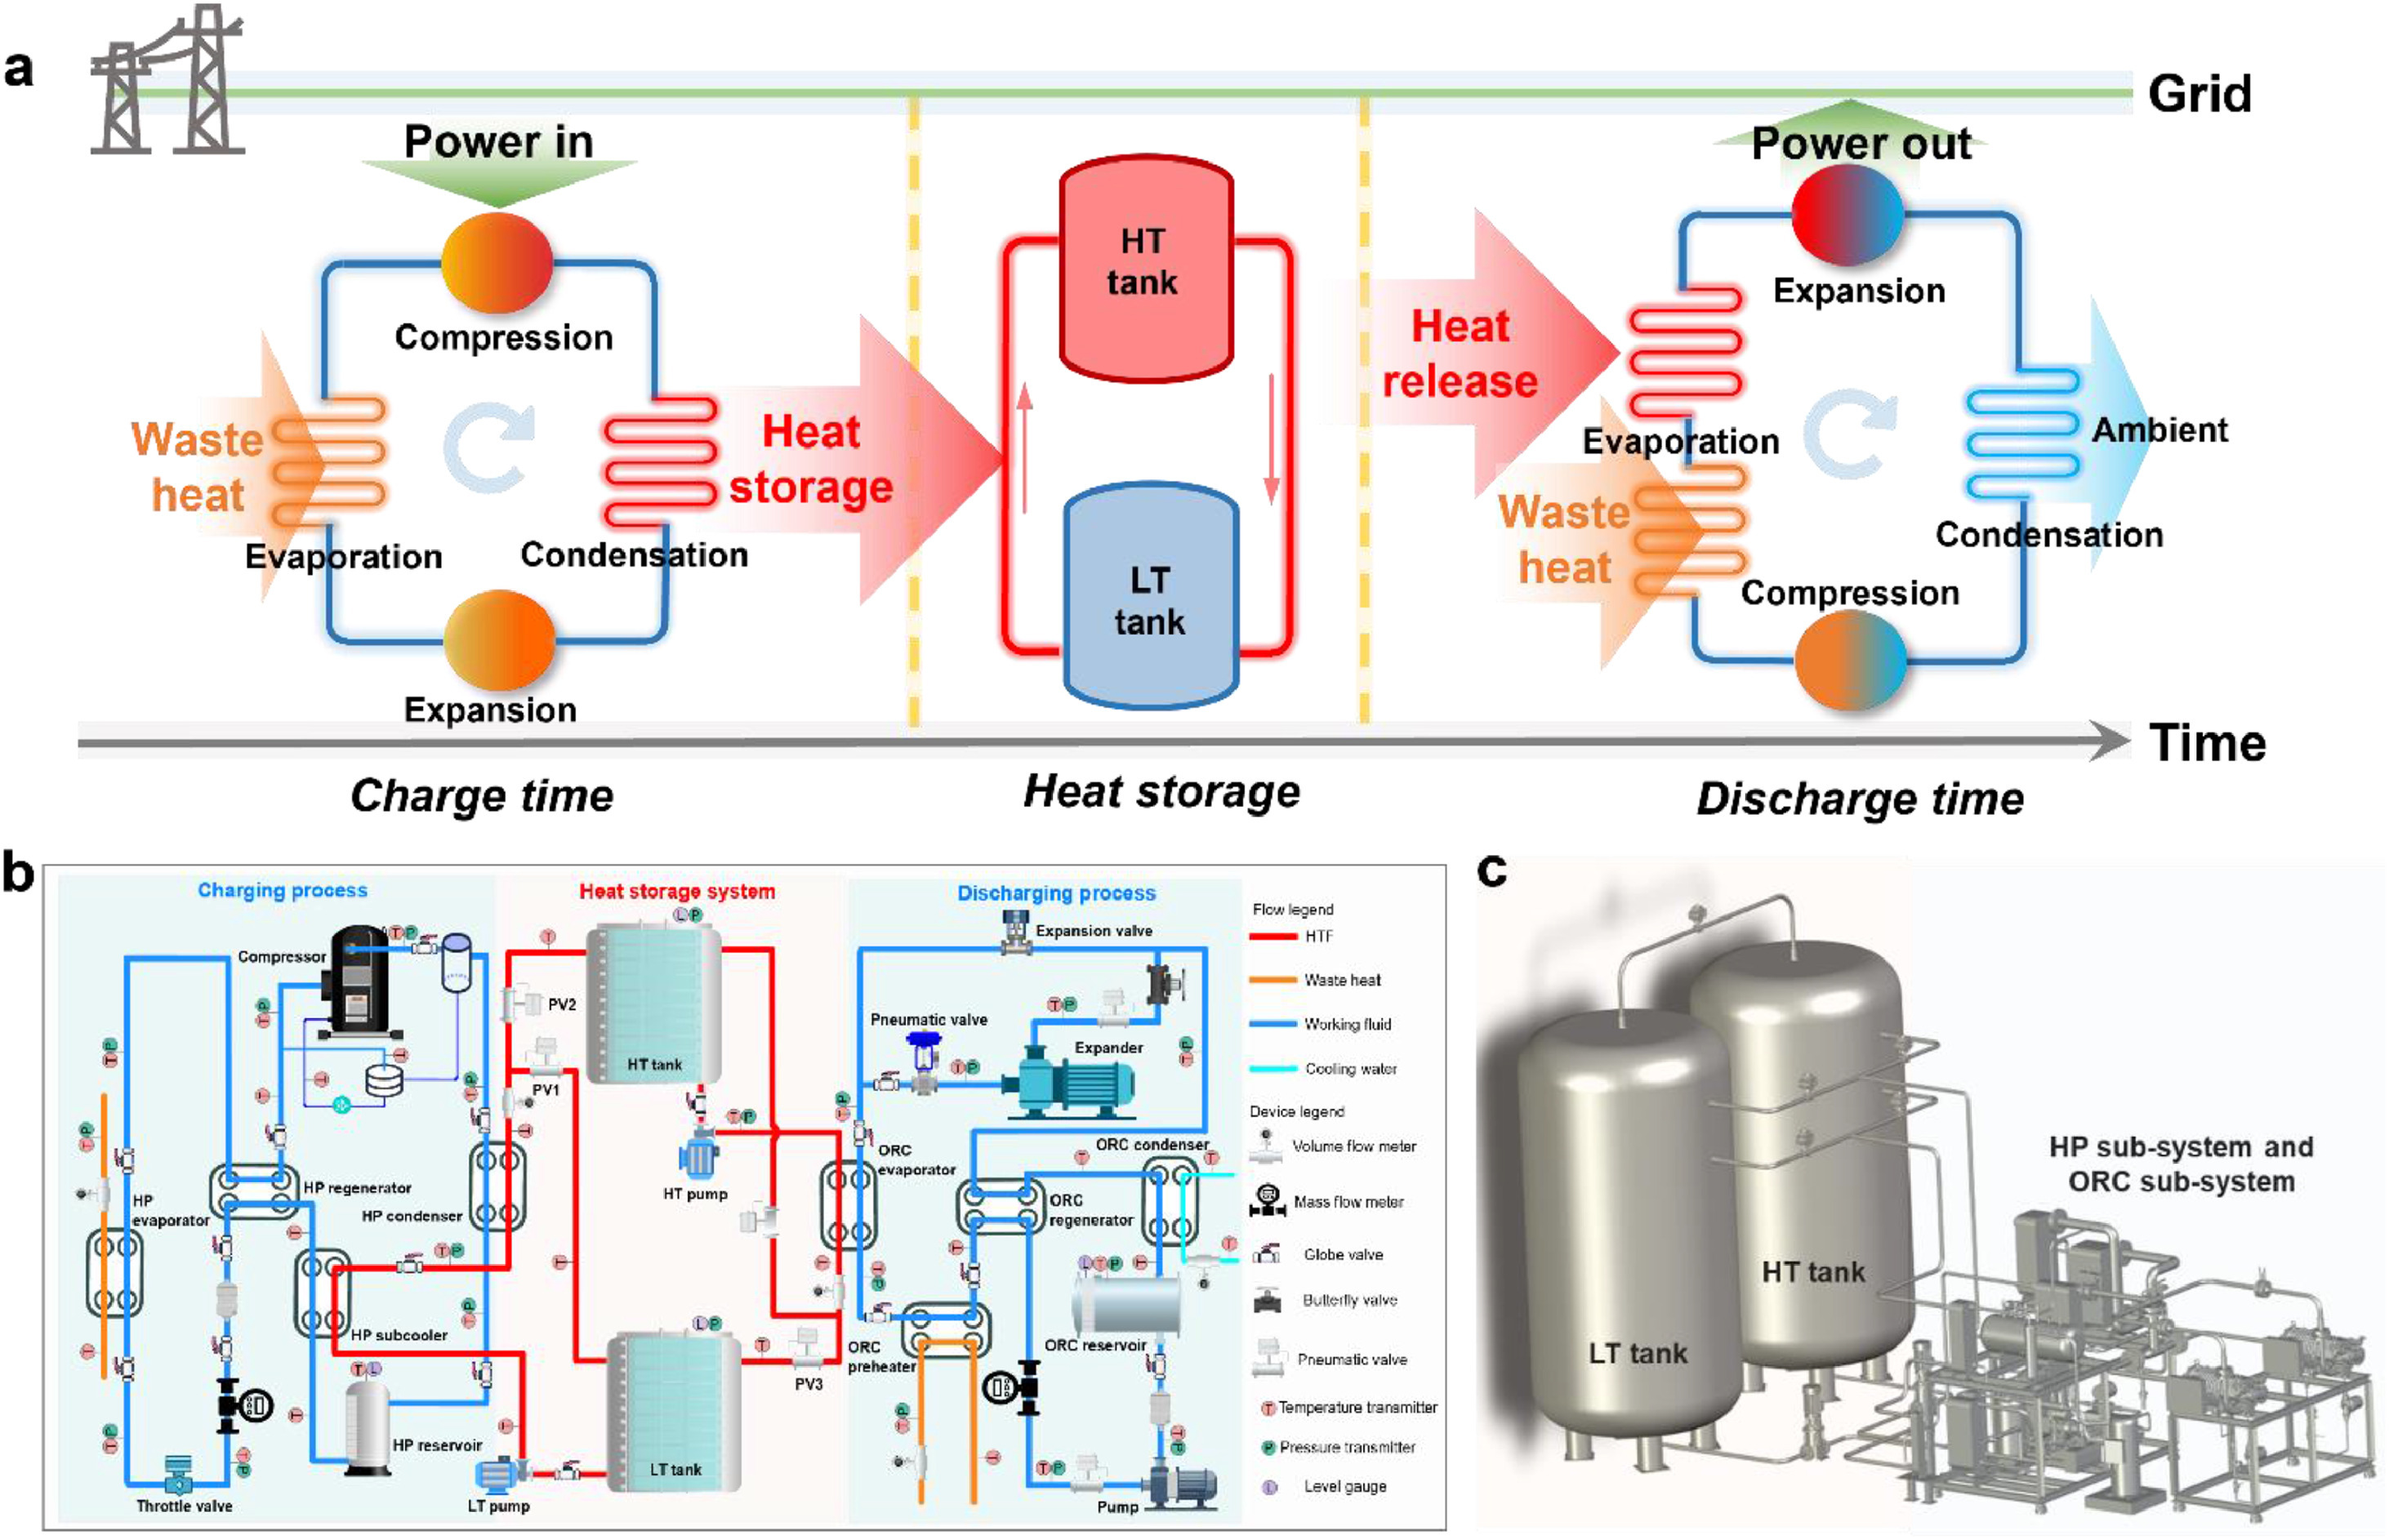
\includegraphics[width=0.8\textwidth]{Abbildungen/CarnotBatterie.jpg}
    \caption{Aufbau einer Carnot Batterie nach \url https://doi.org/10.1016/j.fmre.2026.01.015}
    \label{fig:CarnotBatterie}
\end{figure}


\end{document}
